\documentclass[tikz, margin=2]{standalone}
\usepackage{amsmath}

\begin{document}
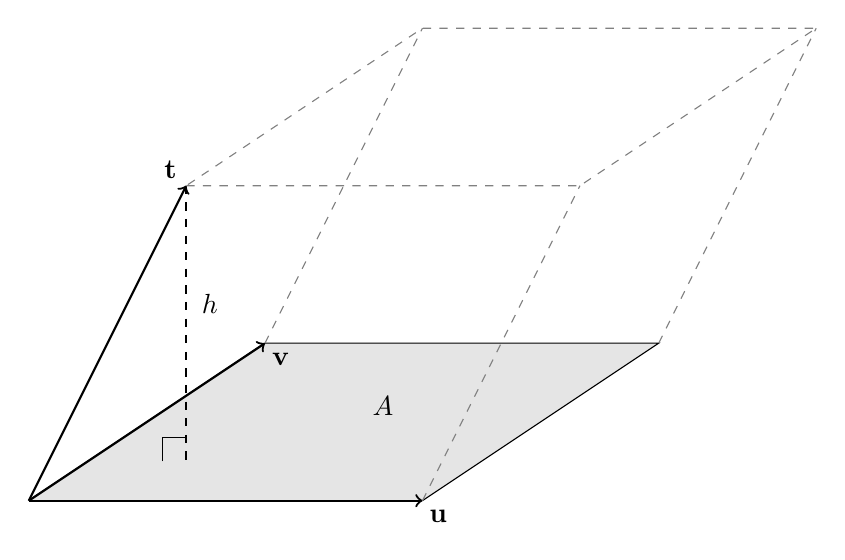
\begin{tikzpicture}

% The parallelogram bounded by u and v
% Draw this first to not be occluded by the vectors
\filldraw[fill=lightgray!40,draw=black] (0,0) -- (5,0) -- (8,2) -- (3,2) -- (0,0);
\node at (4.5,1.2) {\(A\)};

% The vectors u v t and their labels
\draw[color=black,thick,->] (0,0) -- (5,0);
\draw[color=black,thick,->] (0,0) -- (3,2);
\draw[color=black,thick,->] (0,0) -- (2,4);
\node at (5.2,-.2) {\(\mathbf{u}\)};
\node at (3.2,1.8) {\(\mathbf{v}\)};
\node at (1.8,4.2) {\(\mathbf{t}\)};

% The height of the test vector, the right angle, and its label
\draw[color=black,dashed,thick] (2,4) -- (2,.5);
\draw[color=black] (1.7,.5) -- (1.7,.8) -- (2,.8);
\node at (2.3,2.5) {\(h\)};

% The dotted parallelapiped
\draw[color=gray,dashed] (2,4) -- (7,4) -- (10,6) -- (5,6) -- (2,4);
\draw[color=gray,dashed] (8,2) -- (10,6);
\draw[color=gray,dashed] (3,2) -- (5,6);
\draw[color=gray,dashed] (5,0) -- (7,4);

\end{tikzpicture}
\end{document}
